% .:: Laden der LaTeX4EI Formelsammlungsvorlage
\documentclass[fs, footer]{latex4ei}
\usepackage[european]{circuitikz}

\usepackage{multirow}
\usepackage{latexnew}

\renewcommand{\t}{\texttt}
\newcommand{\f}{{\bfseries}}


% Dokumentbeginn
% ======================================================================
\begin{document}


% Aufteilung in Spalten
\vspace{-4mm}
\begin{multicols*}{4}
	\fstitle{Algorithmen und\\ Datenstrukturen}

\iffalse
\subsection{Mengenalgebra}
Potenzmenge: Die Menge aller Teilmengen. $\mathcal P(A) = \iset{U}{U \subseteq A}$\\
Karthesisches Produkt: $A \times B = \iset{(a,b)}{a \in A \land b \in B}$\\
Zwei Mengen $A$ und $B$ heißen disjunkt, wenn $A \cap B = \emptyset$\\

\subsubsection{Relationen}
Eine zweistellige Relation $R$ zwischen zwei Mengen $A$ und $B$ ist eine Teilmenge von $A \times B$\\
Eigenschaften von $R \subseteq A \times B$:
\begin{description}
	\item[reflexiv:] $\forall a \in A: (a,a)\in R$	\qquad $aRa$ (ist wahr) 
	\item[symmetrisch:] $\forall a,b \in A:(a,b) \in R \Rightarrow (b,a) \in R$ \qquad $aRb \Leftrightarrow bRa$
	\item[antisymmetrisch:] $\forall a,b \in A:(a,b) \in R \land (b,a) \in R \Rightarrow a=b$ \qquad $aRb \ \land \ bRa \Rightarrow a=b$
	\item[transitiv:] $\forall a,b, \in A:(a,b) \in R\land (b,c) \in R \Rightarrow (a,c) \in R$ \qquad $aRb \ \land \ bRc \Rightarrow aRc$
\end{description}

$R$ heißt partielle Ordnung, falls $R$ reflexiv, antisymmetrisch und transitiv ist.\\
$R$ heißt Äquivalenzrelation, falls $R$ reflexiv, symmetrisch und transitiv ist.\\
Eine partielle Ordnung heißt totale Ordnung, falls alle Elemente miteinander vergleichbar sind.\\
\fi

\subsection{Allgemeines}
Auf/Abrunden: $x-1 < \lfloor x \rfloor \le x \le \lceil x \rceil < x+1$\\
$\lfloor 3,7 \rfloor = 3$ \qquad $\lceil 3,1 \rceil = 4$ \qquad $\lceil \frac{a}{b} \rceil \le \frac{a+(b-1)}{b}$\\[0.5em]
Modulo \boxed{ a\% n = a\mod n = a - \left(\left\lfloor \frac{a}{n} \right\rfloor \cdot n\right) }\\
Gesucht $r$ mit $a = nq +r$ \qquad $0 \le r < n, q \in \mathbb Z$\\
\\
Fakultät: $n! = \begin{cases} n \cdot (n-1)! & \text{für } n \ge 1 \\ 1  & \text{für } n = 0 \end{cases}$\\
Fibonacci-Zahl: $f(n) = \begin{cases} f(n-1) + f(n-2) & \text{für } n\ge 2\\ 1 & \text{für } n = 1 \\ 0 & \text{für } n = 0 \end{cases}$\\
Fibonacci-Folge: $0,1,1,2,3,5,8,13,21,34,55,89,...$\\
\iffalse
Alphabet $A$: Endliche, nichtleere Menge von Elementen.\\
$(A,<)$ heißt geordnetes Alphabet, wenn $<$ eine totale Ordnung auf A ist.\\
Wort über $A$: $w=a_1 a_2 \ldots a_k$
$A^k := \iset{w}{|w|=k}$\\
$A^{*} = \bigcup\limits_{k=0}^\infty A^k$\\
$A^{+} = \bigcup\limits_{k=1}^\infty A^k$
\fi

\iffalse
\subsection{Newton-Verfahren}
NEWTONS-METHOD$(x_0,f,f',\varepsilon)$\\
$error = \varepsilon + 1$\\
while $error > \varepsilon$\\
	$x_{next} = x -\frac{f(x)}{f'(x)}$\\
	$error = |x_{next} - x|$\\
	$x=x_{next}$\\
return $x$\\
\fi

\section{Algorithmen}
% ==========================================================================================================
Ein Algorithmus ist ein Verfahren mit einer \textbf{präzisen} (d.h. in einer genau festgelegten Sprache
abgefassten) \textbf{endlichen} Beschreibung, unter Verwendung \textbf{effektiver} (tatsächlich ausführbarer), \textbf{elementarer} Verarbeitungsschritte.
Ein Algorithmus besitzt eine oder mehrere Eingaben (Instanz mit Problemgröße $n$) und berechnet daraus eine oder mehrere Ausgaben.\\
Die Qualität eines Algorithmus ergibt sich aus seiner Effizienz, Komplexität, Robustheit und Korrektheit.\\
\\
\subsection{Darstellungsarten}
\begin{itemize}
%TODO Eventuell Bilder
\item Flussdiagramm (Statements als Blöcke, verzweigte Bedingungen)
\item Struktogramm (Pseudocode, Bei Bedingung mehrere Spalten)
\item Programmiersprache/Pseudocode
\end{itemize}
\subsection{Elementare Bausteine}
\begin{itemize}
\item Elementarer Verarbeitungsschritt (z.B. Zuweisung Variable)
\item Sequenz
\item Bedingter Verarbeitungsschritt (if/else)
\item Wiederholung (for/while)
\end{itemize}
\subsection{Eigenschaften}
\textbf{Determiniert:} Der Algorithmus liefert bei gleichen Startbedingungen das gleiche Ergebnis.\\
\textbf{Deterministisch:} Die nächste, anzuwendende Regel ist zu jedem Zeitpunkt definiert.\\
\subsection{Algorithmenmuster (Design Patterns)}
\subsubsection{Divide and Conquer}
Rekursive Rückführung eines zu lösenden Problems auf mehrere identische Probleme mit kleinerer Eingabemenge bis zum Trivialfall\\
\textbf{Beispiele:} Binäre Suche, MergeSort, Quicksort
\subsubsection{Greedy}
Schrittweise Erweiterung der Lösung ausgehend von Startlösung unter Berücksichtigung des bestmöglichsten Schrittes\\
\textbf{Beispiele:} Berechnung Wechselgeld, Glasfasernetz
\subsubsection{Brute Force}
Erzeuge alle in Frage kommenden Kandidaten und suche besten aus\\
\subsubsection{Backtracing}
Systematische Suchtechnik, um Lösungsraum vollständig abzuarbeiten\\
\textbf{Beispiele:} Labyrinth (mit frühem Abbrechen von falschen Lösungspfaden)
\subsubsection{Dynamisches Programmieren}
Statt Rekursion berechnet man vom kleinsten Teilproblem "aufwärts". Zwischenergebnisse werden in Tabellen gespeichert\\
\textbf{Beispiele:} Fibonacci
\subsection{Effizienz}
Die Effizienz eines Algorithmus ist seine Sparsamkeit bezüglich der Ressourcen, Zeit und Speicherplatz, die er zur Lösung eines festgelegten Problems beansprucht.

\subsection{Komplexität}
Schrankenfunktionen:
$1<\log_{10}(n)<\ln(n)<\log_2(n)<\sqrt{n}<n<n\cdot \ln(n)<(\log n)! <n^2 < e^n < n! < n^n < 2^{2^n}$
Aber $\eset{\log_{10}(n), \ln (n), log_2 (n)} \in \Theta(\log n)$

Landau-Symbole:\\
\begin{tabular}{l|ll}
	Notation & Definition\\ \hline
	$f \in \mathcal O \bigl(g(n)\bigr)$ & $0 \le f(n) \le c \cdot g(n)$ & $\forall n > n_0$\\
	$f \in \Omega \bigl(g(n)\bigr)$ & $f(n) \ge c \cdot g(n) \ge 0$ & $\forall n > n_0$\\
	$f \in \Theta \bigl( g(n) \bigr)$ &  $c_1 \cdot g(n) \le f(n) \le c_2 \cdot g(n)$ & $\forall n > n_0$\\
\end{tabular}\\
\subsubsection{Asymptotische Notation}
\begin{tabular}{l|l|l}
Notation & Grenzwertdef. (falls existent) & Wachstum \\
\brule
$g \in \mathcal O (f)$ & $0 \leq \lim_{n \rightarrow \infty}\fr{g(n)}{f(n)} < \infty$ & nicht schneller als $f$\\
$g \in \Omega (f)$ & $0 < \lim_{n \rightarrow \infty}\fr{g(n)}{f(n)} \leq \infty$ & nicht langsamer als $f$\\
$g \in \Theta (f)$ & $0 < \lim_{n \rightarrow \infty}\fr{g(n)}{f(n)} < \infty$ & gleich wie $f$\\
$g \in o(f)$ & $\lim_{n \rightarrow \infty}\fr{g(n)}{f(n)} = 0$ & langsamer als $f$\\
$g \in \omega (f)$ & $\lim_{n \rightarrow \infty}\fr{g(n)}{f(n)} = \infty$ & schneller als $f$\\
\end{tabular}

\subsubsection{Rechenregeln}

$c \cdot f(n) = \mathcal O(f(n))$ für eine beliebige Konst. $c$\\
$\mathcal O(f(n)) + \mathcal O(g(n)) = \mathcal O(f(n) + g(n))$\\
$\mathcal O(f(n)) \cdot \mathcal O(g(n)) = \mathcal O(f(n)g(n))$\\
$\mathcal O(f(n)) + \mathcal O(g(n)) = \mathcal O(max\{f(n),g(n)\})$\\
Gilt auch für $\Omega$ und $\Theta$.

\subsubsection{Typische Laufzeitklassen}
\begin{tabular}{l|l|l}
 & Laufzeittyp & Beispiel \\ \hline
$\Theta (1)$ & konstant & Löschen von erstem El. aus Liste\\
$\Theta (\log n)$ & logarithmisch & Suchen in sortierter Liste \\
$\Theta (n)$ & linear & Suchen in unsortierter Liste\\
$\Theta (n \log n)$ & loglinear & Quicksort\\
$\Theta (n^2)$ & quadratisch & Insertion Sort\\
$\Theta (n^3)$ & kubisch & Matrix-Matrix-Multiplikation\\
$\Theta (2^n)$ & exponentiell & Traveling Salesman\\
\end{tabular}
\textbf{Beispiele:}
\begin{itemize}
	\item Array: elementAt $\mathcal O(1)$, insert $\mathcal O(n)$, erase $\mathcal O(n)$
	\item LinkedList: elementAt $\mathcal O(n)$, insert $\mathcal O(n)$, erase $\mathcal O(n)$
	\item Stack (Array/LinkedList): push, pop, top $\mathcal O(1)$
	\item Queue (LinkedList): push, pop, top $\mathcal O(1)$
\end{itemize}
\subsubsection{Rekurrenzen}
\textbf{Substitutionsmethode:} Lösung raten, einsetzen und mit Induktion beweisen.\\
\\
\textbf{Mastertheorem:}\\
Gegeben: \boxed{ T(n) = a \cdot T\left(\frac{n}{b}\right) + f(n)$ mit $a \ge 1, b > 1 }\\ 
$a\ge1$: Anzahl der Unterprobleme innerhalb einer Rekursionstiefe(meist 1 oder 2) \\
$b>1$: Faktor um den jedes Unterproblem verkleinert ist.\\
$f(n)$: Aufwand der durch Division des Problems und Kombination der Teillösungen entsteht(nicht rekursiver Anteil, von $T(n)$ unabhängig.\\
\begin{itemize}
	\item Falls $f(n) \in \mathcal{O}\left( n^{\log_b a - \varepsilon} \right)$\\
		Dann ist $T(n) \in \Theta\left( n^{\log_b a} \right)$
	\item Falls $f(n) \in \Theta\left( n^{\log_b a} \right)$\\
		Dann ist $T(n) \in \Theta\left( n^{\log_b a} \log(n)\right)$
	\item Falls $f(n) \in \Omega\left( n^{\log_b a + \varepsilon} \right)$\\
		Dann ist $T(n) \in \Theta(f(n))$ 
\end{itemize}

	\subsection{Robustheit}
	Die Robustheit eines Algorithmus beschreibt die Fähigkeit auch bei ungünstigen Eingaben korrekt und effizient zu terminieren. 
	\subsection{Korrektheit}
	Ein Algorithmus heißt korrekt, wenn er für jede Eingabeinstanz mit korrekter Ausgabe terminiert.\\
	Qualitätskontrolle:\\
	\begin{itemize}\itemsep0pt
		\item Überprüfung mit geeigneten Eingabedaten die alle möglichen Fälle testen. Deckt einzelne Fehler auf, aber fehlerfreiheit nicht garantiert.\\
		\item Formaler Beweis mit Hoare-Kalkül etc. meist sehr schwierig.
	\end{itemize}

	\subsection{Rekursion}
	Eine Funktion ruft sich selbst auf bis ein Abbruchereignis eintritt. Danach werden die Rückgabewerte in umgekerhrter Reihenfolge verkettet.\\
	Beispiel Fakultät: $\text{fac}(n) = n \cdot \text{fac}(n-1), \text{fac}(1)=1$\\

%TODO Logische Werte und Verknüpfungen
\iffalse
\section{Primitive (Elementare) Datentypen}
\begin{tabular}{llcc}
		Typ & Speicher & signed & unsigned \\ \hline
		boolean & 1 Byte & $\{0,1\}$ & $-$ \\
		char & 1 Byte & $-128 \ldots 127$ & $0,\ldots ,255$ \\
		short & 2 Byte & $-32768 \ldots 32767$ & $0 \ldots 65535$\\		
		int & 4 Byte & $-2^{31} \ldots 2^{31}-1$ & $0 \ldots 2^{32}-1$\\ 
		long & 8 Byte & $-2^{63} \ldots 2^{63}-1$ & $0 \ldots 2^{64}-1$\\	
		float & 32 Bit & & $-$\\
		double & 64 Bit & & $-$\\
\end{tabular}
	\subsection{Negative Zahlen im Zweierkomplement}
	%TODO Negative Zahlen?
	
	\subsection{Gleitkommadarstellung nach IEEE 754}
	$\text{Wert} = (-1)^s \cdot 2^{e-127} \cdot 1.f$\\
	$s$: Vorzeichen, $e$: Exponent, $f$: Mantisse\\ 
	\\[0.5em]
	Spezialwerte: $\text{Wert} = 0 \Leftrightarrow e=0$ \qquad $\text{Wert} = \infty \Leftrightarrow e=255$ \\
	Bitverteilung(single/double):\\
	\begin{tabular}{|c|c|c|} \hline 
		$s(1)$ & \quad $e(8/11)$ \quad\qquad & \qquad\qquad\qquad\ $f(23/52)$ \qquad\qquad\qquad\qquad \\ \hline
	\end{tabular}
	\textbf{Nachteile:}\\
	\begin{itemize}
		\item Viele Dezimalzahlen haben keine Gleitkommadarstellung
		\item Feste Länge der Mantisse $\Rightarrow$ viele Zahlen nicht darstellbar
		\item Kein Vergleich möglich
		\item Keine Zinsberechnung
	\end{itemize}
\fi

\section{Datenstrukturen}
% ==========================================================================================================
Eine Datenstruktur ist eine \textbf{logische Anordnung} von Daten
mit \textbf{Zugriffs- und Verwaltungsmöglichkeiten} der \textbf{repräsentierten Informationen} über Operationen.\\
Eine Datenstruktur besitzt:
\begin{itemize}\itemsep0pt
	\item Menge von Werten
	\item Literale zum Bezeichnen von Werten
	\item Menge von Operationen auf die Werte
\end{itemize}

\subsection{Stapel (Stack)}
\iffalse
\parbox{4cm}{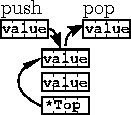
\includegraphics{./img/inf/stack.pdf}}
\pbox{3cm}{\fi
Basieren auf dem LIFO(last in first out) Prinzip.\\
\begin{tabular}{ll}
\t{push(a)}& Legt ein neues Element \t{a} oben auf den Stack\\
\t{pop()}& Entfernt das oberste Element vom Stack\\	
\t{top()}& Gibt das oberste Element vom Stack zurück.\\
\end{tabular}\\
\textbf{Implementierung:} entweder als Array (\t{top()} ist Zeiger auf letztes Element oder als Linked List (Jedes Element zeigt auf das Element darunter)\\
%}

\subsection{Warteschlange (Queue)}
\iffalse
\parbox{4cm}{ 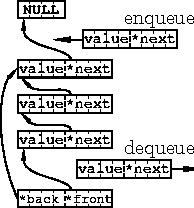
\includegraphics{./img/inf/queue.pdf} }
\pbox{3cm}{\fi
\begin{tabular}{ll}
\t{*front}& zeigt auf das erste Element der Warteschlage\\
\t{*back}& zeigt auf das Ende der Warteschlange.\\
\t{enqueue(x)}& x am Ende der Warteschlange hinzufügen.\\
\t{dequeue()}& Erstes Element aus der Warteschlange nehmen und\\& zurückgeben.\\
\end{tabular}
\textbf{Implementierung} z.B. als abgewandelte Linked List, d.h. Zeiger auf erstes und letztes Element werden gespeichert und jedes Element zeigt auf das nächste.
%}
\iffalse
\begin{multicols*}{2}
ENQUEUE(Q, x)\\
1\ Q[ende[Q]] = x\\
2\ if ende[Q] = länge[Q]\\
3\ \quad then ende[Q] = 1\\
4\ \quad else ende[Q] = ende[Q] + 1\\
\columnbreak \\
DEQUEUE(Q)\\
1\ x = Q[kopf [Q]]\\
2\ if kopf [Q] = länge[Q]\\
3\ \quad then kopf [Q] = 1\\
4\ \quad else kopf [Q] = länge[Q] + 1\\
5\ return x\\
\end{multicols*}
\fi

\textbf{Priority Queue:} Queue mit zugeordnetem Schlüssel, Entfernen von Element mit minimalem Schlüssel, Speicherung in fast vollständigem Binärbaum\\

\subsection{Feld/Liste}
\begin{tabular}{ll}
\t{elementAt(i)}& Element in Position \t{i}\\
\t{insert(d, i)}& Element \t{d} an Position \t{i} einfügen\\
\t{erase(i)}& Element an Position \t{i} entfernen\\
\t{size()}& Gibt Größe/Länge des Feldes zurück\\

\end{tabular}

\subsubsection{Vorteile und Nachteile der Implementierungen}
\begin{tabular}{l|l|l}
DS & Vorteile & Nachteile \\
\brule
Array & direkter Zugriff mit $A[i]$ & Verlängern aufwendig \\
 & sequ. Durchlaufen einfach & Hinzufügen löschen aufwendig \\
\brule
Linked & sequ. Durchlaufen einfach & Zugriff auf i-tes Element\\
List & dynamische Länge & zusätzlicher Speicher für Zeiger\\
 & Einfügen/Löschen einfach & \\
\brule
Double & Durchlauf beide Richtungen & zusätzlicher Speicher für Ptr\\
Linked & Einfügen/Löschen einfacher & Referenzverw. aufändig\\
List & & \\
\end{tabular}

\subsection{Union Find}
Verwaltet die Partitionierung einer Menge in disjunkte Teilmengen.\\
\begin{tabular}{ll}
\t{makeset(x)}& Fügt Element hinzu\\
\t{find(x)}& Findet die Menge, die x enthält\\
\t{union(x, y)}& Die Funktion fügt die beiden Mengen zusammen\\
\end{tabular}
\textbf{Implementierung}: Als Linked List: Set = Liste. Jedes Element zeigt auf auf das nächste Element und zusätzlich auf das Set, in dem es enthalten ist. \t{find()} gibt einfach den Zeiger das enthaltende Set zurück. \t{union()} hängt die beiden Listen aneinander und überschreibt alle Zeiger auf eins der Sets. Auch Baumimplementierung ist möglich.
%TODO Baumimplementierung, Pfadkomprimierung

\subsection{Augmentierung/Abänderung}
\begin{enumerate}
	\item Wähle eine zugrundeliegende Datenstruktur
	\item Welche zusätzliche Information wird gebraucht?
	\item Zeige: Diese Informationen können effizient geupdated werden wenn die Datenstruktur geändert wird
	\item Entwickle die Operationen
\end{enumerate}

\section{Sortieralgorithmen}
in-place: Nur konstanter Hilfsspeicher nötig. $S:\mathcal O(1)$\\
out-of-place: Zusätzlicher Speicher abhängig von $n$ nötig. $S:\mathcal O(f(n))$\\


\subsection{Insertion-Sort}
\begin{enumerate}
	\item Wähle beginnend bei 2 das nächste Element. 
	\item Solange es kleiner als seine Vorgänger ist, tausche es.
\end{enumerate}
Im schlimmsten Fall $\frac{n}{2}(n-1)$\\
\t{INSERTIONSORT(A)\\
1\ for i = 2 to Länge(A) do\\
2\ \quad key $\leftarrow$ A[i]\\
3\ \quad j = i\\
4\ \quad while j $>$ 1 and A[j-1] $>$ key do\\
5\ \qquad 	A[j] = A[j - 1]\\
6\ \qquad 	j = j - 1\\
7\ \quad 	A[j] = key
}

\subsection{Quicksort $\O(n^2)$, avg: $\O(n\log n)$}
\begin{enumerate}
	\item Wähle ein Pivotelement, welches die Liste in zwei Hälften teilt. 
	\item Sortiere die Liste so um, das Elemente die kleiner als das Pivotelement in der einen Hälfte und größere in der anderen Hälfte sind. 
		Suche dazu mit zwei Laufvariablen das Feld ab, bis jede eine unpassende Variable gefunden hat, dann tausche diese.
	\item Wiederhole die Schritte 1. bis 3. mit beiden Teillisten, bis jede Teilliste sortiert ist.
\end{enumerate}

\parbox{4cm}{
\t{QUICKSORT (A, p, r)\\
1\ if p $<$ r \{\\
2\ \quad q = PARTITION (A, p, r)\\
3\ \quad QUICKSORT (A, p, q - 1)\\
4\ \quad QUICKSORT (A, q + 1, r)\\
5\ \}
}}\hspace{-.5cm}
\parbox{4cm}{
\t{PARTITION(A, p, r)\\
1\ x = A[r] //Pivotelement\\
2\ i = p-1 \\
3\ for j = p to r - 1 \{\\
4\ \quad if A[j] $\le$ x \{\\
5\ \qquad i = i+1\\
6\ \qquad vertausche A[i] $\leftrightarrow$ A[j]\\
7\ \quad \}\\
8\ \}\\
9\ vertausche A[i + 1] $\leftrightarrow$ A[r]\\
10\ return i + 1\\}}

\subsection{Mergesort $T(n) = 2T(\fr{n}{2}) + \O(n) \Rightarrow \O(n\log n)$}
Feld in der Mitte rekursiv halbieren, bis Feldlänge = 1\\
Teilsortierte Felder zusammenfügen(Reißverschluss)\\

\parbox{4.5cm}{
\t{mergeSort(List* a)\\
1.	if (a$\rightarrow$length() $<$= 1)\\
2.	\quad return a;\\
2.	List* b = a$\rightarrow$half();\\
3.	a = mergeSort(a);\\
4.	b = mergeSort(b);\\
5.	return merge(a,b);\\
\\
half()\\
1.	Node* ptr = head;\\
2.	for (0 bis length/2-2)\\
3.	\quad ptr = ptr$\rightarrow$next;\\
4.	List* L = new List(ptr$\rightarrow$next);\\
5.	ptr$\rightarrow$next = NULL;\\
6.	return L;
}}\hspace{-1.25cm}
\parbox{3.5cm}{
\t{\textit{elAt() entspricht elementAt()}
merge(a, b)\\
1.	if (a$\rightarrow$empty())\\
2.	\quad delete a; return b;\\
3.	if (b$\rightarrow$empty())\\
4.	\quad delete b; return a;\\
5.	List* h;\\
6.	if a$\rightarrow$elAt(0) $<$ b$\rightarrow$elAt(0)\\
7.	\quad h = a; else h = b;\\
8.	int d = h$\rightarrow$removeFront();\\
9.	List L = merge(a,b);\\
10.	L$\rightarrow$insertFront(d);\\
11.	return L;\\
}}

\iffalse
\subsection{Heapsort}

\begin{multicols}{2}

HEAPSORT (A)\\
1.  BUILD-MAX-HEAP (A)\\
2.  for i = länge [A] downto 2\\
3. 	do vertausche A [1] <-> A[i]\\
4. 	heap-größe [A] = heap-größe [A] -1\\
5.	MAX-HEAPIFY (A,1)\\
\\
BUILD-MAX-HEAP (A)\\
1.  heap-größe [A] = länge [A]\\
2.  for i = $\lfloor$ länge [A] /2 $\rfloor$ downto 1\\
3.  \quad MAX-HEAPIFY (A,i)\\
\columnbreak \\
MAX-HEAPIFY (A, i)\\
1.  l = LEFT (i)\\
2.  r = RIGHT (i)\\
3.  if l <= heap-größe [A] und A[l] $>$ A[i]\\
4. 	\quad maximum = l\\
5. 	else maximum = i\\
6.  if r <= heap-größe [A] und A[r] $>$ A [maximum]\\
7.  \quad maximum = r\\
8.  if maximum $\neq$ i\\
9.  \quad vertausche A[i] $\leftrightarrow$ A [maximum]\\
10. \qquad MAX-HEAPIFY (A, maximum)\\

\end{multicols}
\fi

\subsection{Laufzeiten und Speicherbedarf von Sortieralgorithmen}
Die Laufzeit bzw. Taktzyklen in Abhängigkeit einer (meist großen) Eingabemenge $n$.\\
\begin{tabular}{l|l|l|l|l}
	Name & Best & Avg & Worst & Zusätzlicher\\
	 & & & & Speicher\\ \hline
	Selection & $\mathcal O (n^2)$ & $\mathcal O (n^2)$ & $\mathcal O (n^2)$ & in-place\\
	Insertion & $\mathcal O (n)$ & $\mathcal O (n^2)$ & $\mathcal O (n^2)$ & in-place\\
	Bubblesort & $\mathcal O (n)$ & $\mathcal O (n^2)$ & $\mathcal O (n^2)$ & in-place\\
	Merge & $\mathcal O (n \cdot \log_2 n)$ & $\leftarrow$ & $\leftarrow$ & $\mathcal O (n)$\\ %$n \cdot \lceil  \log_2 n \rceil$\\
	Heap-Sort & $\mathcal O (n \cdot \log_2 n)$ & $\leftarrow$ & $\leftarrow$ & in-place\\	
	Quick & $\mathcal O (n \cdot \log_2 n)$ & $\leftarrow$ & $\mathcal O (n^2)$ & in-place\\
\end{tabular}\\
in-place bedeutet zusätzlicher Speicher von $\mathcal O (1) = \text{const.}$\\
Vergleichende Sortieralgorithmen brauchen mindestens $\Omega(n \log_2 n)$ Vergleiche, egal wie clever sie sind!





\subsection{Suchalgorithmen}
\textbf{sequentielles Suchen:} Feld durchlaufen und vergleichen\\
Laufzeit: $\mathcal O(n)$, geeignet für statische kleine Mengen\\
\textbf{binäres Suchen:} Vorsortieren, Vergleich mit Mitte\\
Laufzeit: $\mathcal O(\log n)$, geeignet für statische große Mengen\\
\textbf{binärer Suchbaum} für dynamische Mengen\\

\iffalse
	\subsection{String-matching}
	In einer Zeichenfolge $T[0 ... n]$ wird ein Muster $P[0...m]$ gesucht.\\ 
	\\
	Rabin-Karp Algorithmus: Jedes Zeichen wird als Zahl interpretiert.\\
	Muster $p = P[m] + 10 P[m-1] + ... + 10^i P[m-i]$\\
	- Bilde modulu mit einer Primzahl $q$ (Vorfiltern): $T[s ... s+m] \% q$\\
	- Bei Übereinstimmung des Restes: genauere Prüfung.\\
	Laufzeit: $\mathcal O(m+n)$ bei $m<<n$: $\mathcal O(n)$\\
\fi




\section{Graphen}
% ==========================================================================================================
$G = (E, V)$, mit E: Kanten, V: Knoten\\
\textbf{Adjazenzmatrix} $(V \times V)$: $1$ oder $0$ für Verbindung oder Gewicht.\\
Bei ungerichtetem Graph symmetrisch, sinnvoll wenn Graph fast vollständig\\
\textbf{Adjazenzliste:} Für jeden Knoten alle Nachbarknoten angeben mit Startknoten $s$\\

\textbf{Ungerichteter Graph:} Richtung der Kante spielt keine Rolle\\
\textbf{Gerichteter Graph:} Richtung der Kante spielt eine Rolle, Schleifen möglich $(u, u)$ mit $u \in V$\\

\subsection{Eigenschaften}
$v$ \textbf{adjazent} zu $u$: $(u,v) \in E$ bzw. $\{u, v\} \in E$ für $u, v \in V$\\
\textbf{Inzident}: Knoten $v$ und Kante $e = (x, v)$ bzw. $e = \{x, v\}$ mit $v, x \in V$\\

Pfad: Folge von miteinander verbundenen Knoten\\
einfacher Pfad: alle Knoten sind paarweise verschieden\\
Zyklus: Pfad mit gleichem Anfangs- sowie Endknoten\\
Kreis: einfacher Pfad mit gleichem Anfangs- sowie Endknoten\\

\subsubsection{Gerichteter Graph}
Anzahl der eintretenden Kanten in $v$ heißt Eingangsgrad: $indeg(v)$\\
Anzahl der austretenden Kanten aus $v$ heißt Ausgangsgrad: $outdeg(v)$\\

stark zusammenhängend: jeder Knoten ist von jedem anderen Knoten erreichbar\\
starke Zusammenhangskomponente: stark Zusammenhängender Teilgraph\\

\parbox{3.6cm}{
	Gibt alle zusammenhängenden\\ Komponenten eines gerichteten\\ Graphen aus\\
	\t{dfsTarjan()\\
	1.	dfsCount = 1;\\
	2.	foreach v $\in$ V\\
	3.	\quad v->state = initial;\\
	4.	\quad v->parent = NULL;\\
	5.	foreach s $\in$ V\\
	6.	\quad if (s->state == initial)\\
	7.	\quad \quad dfsVisitTarjan(s)\\
}}\hspace{-.2cm}
\parbox{3.5cm}{\t{dfsVisitTarjan(v) \\
	1.	v->state = active;\\
	2.	v->num = dfsCount++;\\
	3.	\$.push(v);\\
	4.	foreach (x $\in$ N[v])\\
	5.	\quad if (x->state == initial)\\
	6.	\quad \quad x->parent = v\\
	7.	\quad \quad dfsVisitTarjan(x);\\
	8.	if (cut parent edge of v)\\
	9.	\quad repeat\\
	10.	\quad \quad x = \$.pop();\\
	11.	\quad \quad // add x to current component\\
	11. \quad until (v == x) \\
	12. \quad // print current component\\
}}

\subsubsection{Ungerichteter Graph}
Anzahl der Kanten an $v$ heißt Grad: $deg(v)$\\

zusammenhängend: jeder Knoten ist von jedem anderen Knoten erreichbar\\

	\subsection{Minimaler Spannbaum}
	Kruskal-Algorithmus ($\O(m\log n)$):
	\begin{enumerate}\itemsep-2pt
		\item Sortiere alle Kanten aufsteigend nach Gewicht.
		\item Wähle immer die nächst schwerere Kante, wenn sie keine Schleife bildet.
	\end{enumerate}
	
	\parbox{3.6cm}{
	\t{PrimMST(s) \\
	1.	S = new PriorityQueue()\\
	2.	foreach v $\in$ V\\
	3.	\quad v$\rightarrow$key = $\infty$\\
	4.	\quad v$\rightarrow$par = NULL;\\
	5.	\quad v$\rightarrow$han = S$\rightarrow$insert(v);\\
	6.	s$\rightarrow$key = 0;\\
	7.	S$\rightarrow$decreaseKey(s$\rightarrow$han, 0);\\
	}}\hspace{-.2cm}
	\parbox{3.5cm}{
	\t{8.	while(!S$\rightarrow$empty())\\
	9.	\quad v = S$\rightarrow$extractMin();\\
	10.	\quad foreach x $\in$ N[v]\\
	11.	\quad \quad if (x$\rightarrow$key > w(v,x))\\
	12.	\quad \quad \quad S$\rightarrow$decreaseKey(x$\rightarrow$han, \\
	. \quad \quad \quad \quad \quad w(v,x));\\
	13.	\quad \quad \quad x$\rightarrow$key = w(v,x);\\
	14.	\quad \quad \quad x$\rightarrow$par = v;\\
	}}
	
	\subsection{Kürzeste Wege}
	SSSP (single source shortest path)\\
	APSP (all pairs shortest path)\\
	\framebox{ Satz: Teilpfade von kürzesten Pfaden sind auch kürzeste Pfade! }\\
	\textbf{Dijkstra-Algorithmus:} nur positive Kantengewichte!\\
	Menge $S$: Knoten mit dem Gewicht ihres kürzesten Pfades von $s$\\
	Menge $Q$: Min-Prioritätswarteschlange mit den ungeprüften Knoten.\\ 
	Relaxationsschritt: Überprüfe ob ein Umweg über einen anderen Knoten kürzer ist.\\
	Muss für jede Kante nur genau einmal überprüft werden.

	\parbox{3.6cm}{
	\t{BELLMANFORD(s) \\
	Laufzeit: $\O(m\cdot n)$\\
	1.	foreach $v \in V$\\
	2.	\quad	v$\rightarrow$key = $\infty$;\\
	3.	\quad	v$\rightarrow$par = NULL;\\
	4.	s$\rightarrow$key = 0;\\
	5.	for i = 1 to n-1\\
	6.	\quad	foreach (x,y) $\in$ E\\
	7.	\quad \quad		if (y$\rightarrow$key $>$ x$\rightarrow$key + w(x,y))\\
	8.	\quad \quad \quad			y$\rightarrow$key = x$\rightarrow$key + w(x,y);\\
	9.	\quad \quad \quad			y$\rightarrow$par = x;\\
	10.	foreach (x,y) $\in$ E\\
	11.	\quad	if (y$\rightarrow$key $>$ x$\rightarrow$key + w(x,y))\\
	12.	\quad \quad		y$\rightarrow$par = x;\\
	\ \\
	mark(x)\\
	1.	if (x$\rightarrow$key != -$\infty$)\\
	2.	\quad	x$\rightarrow$key = -$\infty$;\\
	3.	\quad	for ((x,y) $\in$ E) mark(y)\\
	}}\hspace{-.2cm}
	\parbox{3.5cm}{
	\t{APSP - Floyd Warshall \\
	Laufzeit: $\O(m\cdot n^2)$\\
	1.	foreach (u,v) $\in$ V\\
	2. \quad	d[u,v] = $\infty$\\
	3. \quad	pred[u,v] = NULL;\\
	4.	foreach v $\in$ V\\
	5. \quad	d[u,v] = 0;\\
	6.	foreach (u,v) $\in$ E\\
	7. \quad	d[u,v] = w(u,v);\\
	8. \quad	pred[u,v] = u;\\
	9.	foreach v $\in$ V\\
	10. \quad	for \{u,w\} $\in$ V $\times$ V\\
	11. \quad \quad	if (d[u,w] $>$ d[u,v] + d[v,w])\\
	12.	\quad \quad \quad	d(u,w) = d(u,v) + d(v,w);\\
	13. \quad \quad \quad	pred(u,w) = pred(v,w);\\
	}}

\subsection{Bäume}
... sind spezielle Graphen mit einer Wurzel, Zweigen und Blätter.\\
Er besitzt keine zyklischen Strukturen und ist zusammenhängend.\\

Begriffe:\\
\textbf{Grad} deg(v): Anzahl der Unterbäume(Äste)\\
\textbf{Blatt:} Knoten mit $deg(v) = 0$\\
\textbf{Tiefe} $d(v)$: Länge des Pfades von der Wurzel bis zum Knoten $v$.\\ 
\textbf{Höhe} $h(v)$: Längster Pfad von $v$ zu einem Blatt.\\   
\textbf{Niveau:} Knoten mit gleicher Tiefe.\\

\subsection{Binärer Suchbaum (BSB)}
... ist ein geordneter Baum und $\forall v \in V:deg(v) \le 2$\\
Ein Binärbaum ist vollständig, wenn $\forall v: deg(v) = 2 \ \lor \ deg(v)=0$\\ 
Falls Höhe $k$, dann gilt: $2^{k+1} - 1$ Knoten und $2^k$ Blätter.\\ 
\\
Bedeutung: Verdopllung der Eingabegröße, mit logarithmischer Vergrößerung der Struktur.\\
Binärbaum als verkettete Liste: Knoten $x$ mit $links[x],rechts[x], parent[x], key[x]$\\

Balancierter Suchbaum: Höhe des Baumes ist immer in $\mathcal O(\log n)$\\
\subsubsection{AVL-Baum}
Betrag der Differenz der Höhe der Teilbäume für jeden Knoten ist $\leq$ 1.\\
AVL-Baum der Höhe $h$ enthält mindestens $F_{h+2}-1$ und höchstens $2^h - 1$ Knoten.
Blattknoten sind Dummys ohne Daten. Jeder interne Knoten hat genau zwei Kinder
Jeder Knoten speichert die Balance $v = h(\text{linkes Kind}) - h(\text{rechtes Kind})$\\
\textbf{Rotationen:}\\
\parbox{.5\linewidth}{
Nach Links: Rechtes Kind wird Wurzel, Wurzel wird linkes Kind der neuen Wurzel, Altes linkes Kind der neuen Wurzel wird rechtes Kind der alten Wurzel.}\parbox{.5\linewidth}{\vspace{-.3cm}
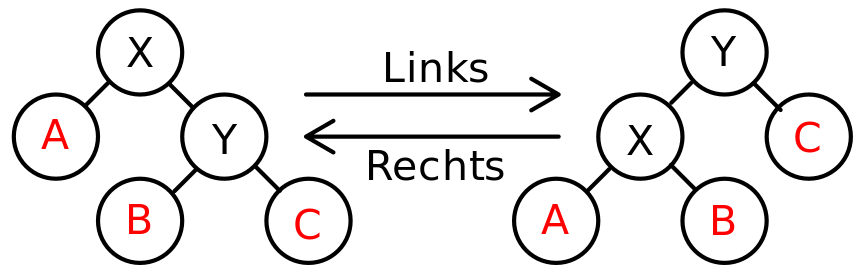
\includegraphics[width=\linewidth]{img/avl-rotate}}\\
Nach Rechts: Umkehrung der Rotation nach links\\
\textbf{Einfügen:}\\
1. Knoten einfügen wie in normalen BSB\\
2. Vom Elternknoten des eingefügten Knotens aufsteigend die Balance aller Knoten bis zur Wurzel prüfen und bei bedarf die AVL-Bedingung wiederherstellen\\
\textbf{Löschen:}\\
1. Knoten löschen wie im normalen BSB\\
2. Vom Elternknoten des überbrücken Knotens aufsteigend die Balance aller Knoten bis zur Wurzel prüfen und bei Bedarf die AVL-Bedingung wiederherstellen\\
\textbf{Balance eines Knoten wiederherstellen:}\\
\t{
 1\ Balance(v)\\
 2\ if (v->balance == -2)\\
 3\ \quad if (v->right->balance $\in \{0, -1\}$)\\
 4\ \qquad   v = LeftRotate(v)\\
 5\ \quad else\\
 6\ \qquad   v->right = RightRotate(v->right)\\
 7\ \qquad   v = LeftRotate(v) // Doppelrotation\\
 8\ else\\
 9\ \quad if (v->left->balance $\in \{0, 1\}$)\\
10\ \qquad   v = RightRotate(v)\\
11\ \quad else\\
12\ \qquad   v->left = LeftRotate(v->left)\\
13\ \qquad   v = RightRotate(v) // Doppelrotation\\
14\ return v\\
}

\subsubsection{Traversierung}
Pre-order: Wurzel $\rightarrow$ linker Teilbaum $\rightarrow$ rechter Teilbaum\\
In-order: linker Teilbaum $\rightarrow$ Wurzel $\rightarrow$ rechter Teilbaum\\
Post-order: linker Teilbaum $\rightarrow$ rechter Teilbaum $\rightarrow$ Wurzel\\

\subsection{Suchen in Graphen}
\textbf{Breitensuche(BFS)} $\Theta (\abs V + \abs E)$\\
Von einem Startknoten $S$ werden alle noch nicht durchsuchten Knoten mit Abstand $k$ durchsucht. Der Suchradius breitet sich aus. Neue Knoten kommen in eine Queue an zu besuchenden Knoten.\\
Code ähnlich wie DFS, nur Stack durch Queue ersetzt.\\
 \\
\textbf{Tiefensuche(DFS)} $\Theta (\abs V + \abs E)$\\
Von einem Knoten werden alle Nachfolger rekursiv durchsucht. Mehrere Verzweigungsmöglichkeiten werden zwischengespeichert.\\
1. DFS(G): Suche im Graph G den nächsten unbesuchten Knoten $a$. Rufe DFS-VISIT(a) auf.\\
2. DFS-VISIT(a): Finde rekursiv alle Nachfolgerknoten von $a$ und markiere sie als durchsucht.\\

\subsection{Heap}
%TODO Bild von Baum einfügen
Fast vollständiger Binärbaum mit Indizierung von links nach rechts und von oben nach unten.
Wert eines Knotens ist immer kleiner bzw. größer als Werte der Kinder. 
Max-Heap: Wurzel hat den größten Wert, Min-Heap: Wurzel hat den kleinsten Wert.\\
\textbf{Heap-Sort:}\\
1. Erzeuge Max-Heap aus $A$\\
2. Wähle $|A| / 2$ als Starknoten, da größter Knoten mit $deg > 1$\\
3. Betrachte Knoten $i$ und seine beiden Kinder $2i$ und $2i+1$ \\

\section{Hashtabellen}
	... sind Felder bei denen die Position eines Objekts durch eine Hashfunktion berechnet wird. Da es zu Kollisionen kommen kann, werden in den Feldern nur Verweise auf eine Liste gespeichert.

	Schlüssel: wird von einem Schlüsselgenerator aus den Daten generiert. 
\subsection{Hashfunktion}
	... ordnet jedem Schlüssel aus einer großen Schlüsselmenge einen möglichst eindeutigen Wert aus einer kleineren Indexmenge zu.
	$h: key \ra index$
	
Operatoren:
Verkettete Hashtabelle: Jedes Feld entspricht einer Liste die mehrere kollidierte Daten speichern kann. 
\begin{description}
	\item[chained-hash-insert(T,x)]: Füge $x$ an den Kopf der Liste $T[ h(x.schluessel)]$
	\item[chained-hash-search(T,k)]: Suche Element $k$ in der Liste $T[ h(k) ]$
	\item[chained-hash-delete(T,x)]: entferne $x$ aus der Liste $T[h(x.schluessel)]$
\end{description}

\section{Fouriertransformation}
Transformation eines periodischen Signals aus dem Zeit in den Frequenzbereich $\rightarrow$ Darstellung als Überlagerung von Sinus- und Kosinusfunktionen\\
\textbf{Theorem:}\\
Jede periodische Funktion $x(t)$ mit Periode $T$ lässt sich als $\sum_{i=-\infty}^\infty \alpha_i e^{j\frac{2\pi}{T}t}$
\subsection{Diskrete Fouriertransformation (DFT)}
Fouriertransformation ist Integration über alle komplexen Exponentialfunktionen $\Rightarrow$ Näherung über Summe entlang des Einheitskreises (mit $n-ten$ Einheitswurzeln)\\
\textbf{Geg.:} $x_0, ..., x_{N-1}$ mit $x_k = x(\frac{T}{N}k)$.
Berechne \[\hat{x}_l = \dfrac{1}{N} \sum_{k=0}^{N-1}x_ke^{-j\frac{2\pi}{N}lk}\quad\forall l \in \{0,...,N-1\}\]
$\Rightarrow$ DFT ist Polynomauswertung, einfache Implementierung $\O(n^2)$
\subsection{Fast Fourier Transform (FFT)}
Schnelle Polynomauswertung mit $N=2^k$.\\
Input: Polynom P vom Grad N-1, Koeffizenten C\\
Output: $R[l]$ enthält $P[W_N^l]$\\
\t{
FFT($C,N,W_N$)\\
1\qquad if ($N$ == 1) return C\\
2\qquad $C_\text{odd} = [C[1], C[3], ..., C[N-1]]$\\
3\qquad $C_\text{even} = [C[0], C[2], ..., C[N-2]]$\\
4\qquad $R_\text{odd}$ = FFT($C_\text{odd}$, $N/2$, $W_N^2$)\\
5\qquad $R_\text{even}$ = FFT($C_\text{even}$, $N/2$, $W_N^2$)\\
6\qquad $W = 1$; // = $W_N^0$\\
7\qquad for $l = 0$ to $N/2-1$\\
8\qquad \qquad $R[l] = R_\text{even}[l] + W * R_\text{odd}[l]$\\
9\qquad \qquad $R[l + N/2] = R_\text{even}[l] - W * R_\text{odd}[l]$\\
10\quad\  \qquad $W \ *\!\!= W_N$; // $= W_N^l$\\
11\quad\  return $R$;\\}
Für DFT: $W_N = e^{-j\frac{2\pi}{N}}$ und Ergebnis durch $N$ dividieren; $\O(n \log n)$

\iffalse
\section{Entropie}
% ==========================================================================================================
... ist ein Maß für den mittleren Informationsgehalt bzw. Informationsdichte eines Zeichensystems(Alphabet).\\
Seltene Zeichen haben einen hohen Informationsgehalt.\\
Das $i$-te Zeichen $z_i$ mit Auftrittswahrscheinlichkeit $p_i$:\\
Informationsgehalt  $I(z_i) = -\log_2(p_i)$\\

	\subsection{Kompression}
	Huffmancode: Wahrscheinliche Zeichen werden mit weniger Bit kodiert als seltene. (z.B UTF-8)\\
	Verschmelze die beiden unwahrscheinlichsten Zeichen zu einem Teilbaum, der Vater bekommt die Summe als Wahrscheinlichkeit.
	
	
	Kommt in Klausur dran: Huffmancode!!!
\fi	
\end{multicols*}
\end{document}